\en

\section{Tool Functionalities}
\label{subsec:func}

We propose three main functionalities for the user in the tool, called the \textbf{Duplication Explorer}, \textbf{Function Information}, and \textbf{Duplication Report}. Each functionality accepts specific parameters to perform its operations, with an optional parameter shared by all: \textbf{minimum similarity per query}. This minimum similarity per query is distinct from the minimum similarity setting introduced in Section \ref{subsec:setup}, as it enables a dynamic adjustment of the similarity threshold within a query-specific context. Below is an explanation of each of these main functionalities.

\subsection{Duplication Explorer}

The Duplication Explorer is the primary functionality of our tool, designed to present the user with pairs of duplicated functions identified by the tool. We implement optional filters to facilitate more complex queries, as described below. Figure \ref{fig:explorer_ex} demonstrates an example of this functionality in use.

\begin{figure}
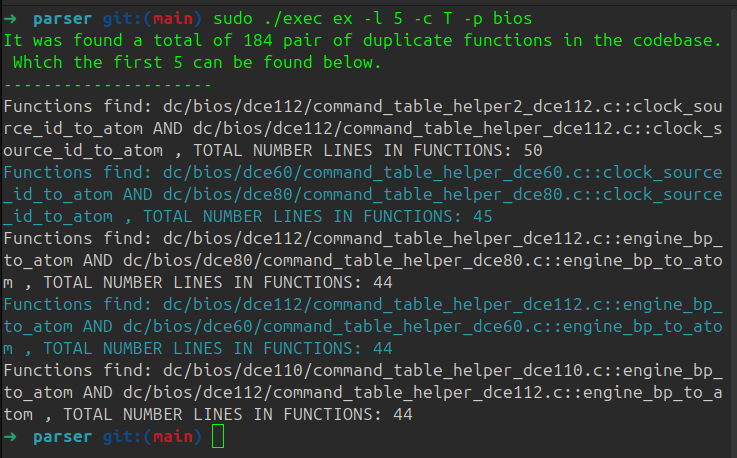
\includegraphics[scale=0.30]{explorer_example}
\caption{Example of the \textit{Duplication Explorer} functionality of the ArKanjo tool in action.}
\label{fig:explorer_ex}
\end{figure}

\begin{itemize}
	\item \textbf{Sorting Filter:} This filter allows the user to sort the results by the similarity score of the function pairs or by the number of duplicated lines. By default, the tool sorts results by similarity, but the user can pass a sorting parameter to switch the sorting method.

	\item \textbf{Limiter Filter:} This filter accepts a numerical parameter, called a limiter, which restricts the number of results displayed to the user to the specified number.

	\item \textbf{Pattern Filter:} This filter allows the Duplication Explorer to ignore duplicated function pairs that do not match a user-defined pattern. A function matches a pattern if the string is formed by concatenating the relative path of the code file with the function name, which contains the pattern as a substring. The user can specify whether both functions in the pair must match the pattern or if matching one of the functions is sufficient.
\end{itemize}

\subsection{Function Information}
\label{subsec:functioncommand}

The purpose of the Function Information functionality is to provide detailed information about a specific function. The functionality receives a target function from the user and returns information such as the relative path, function name, and line numbers where the function is defined. Additionally, it provides similar information for every function that duplicates the given function.

\begin{figure}
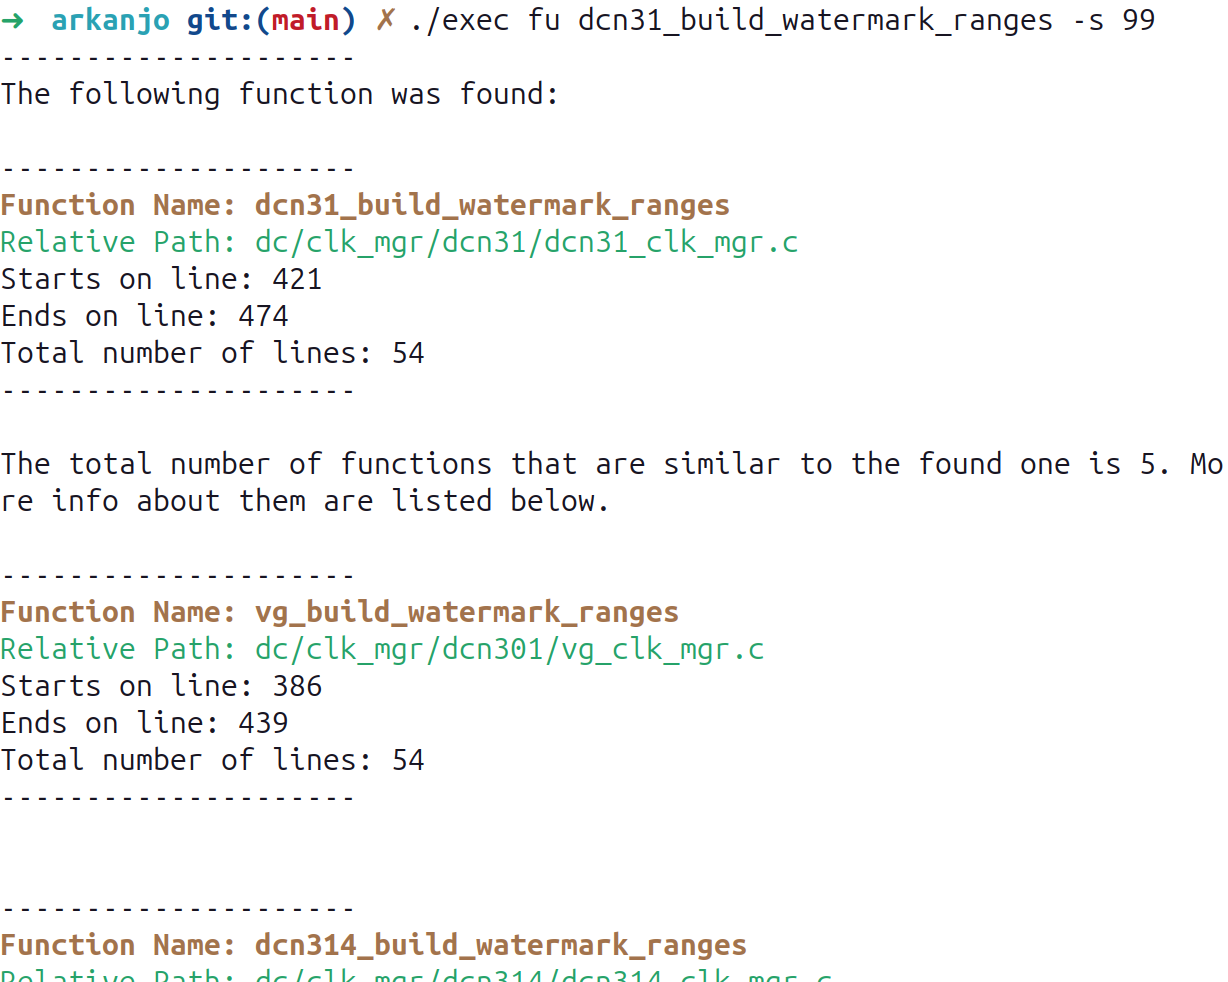
\includegraphics[scale=0.3]{function_example}
\caption{Example of the \textit{Function Information} functionality of the ArKanjo tool in action.}
\label{fig:function_ex}
\end{figure}

Since multiple functions with the same name may exist in a codebase, the user can provide a pattern string to differentiate them. A function matches a pattern if the concatenated string of the relative path and function name contains the pattern as a substring. Figure \ref{fig:function_ex} demonstrates this functionality in action.

\subsection{Duplication Report}

The purpose of the Duplication Report functionality is to provide an overview of duplicated code within the input codebase. This functionality calculates the number of duplicated lines per folder in the codebase and presents the information to the user in a readable format. 

\begin{figure}
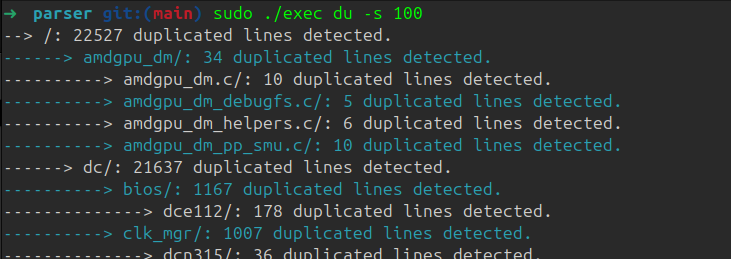
\includegraphics[scale=0.3]{relatory_example}
\caption{Example of the \textit{Duplication Report} functionality of the ArKanjo tool in action.}
\label{fig:relatory_ex}
\end{figure}

The tool utilizes the Code Duplication Database to list duplicated functions and the temporary codebase to determine the line count for these functions to generate this report. Figure \ref{fig:relatory_ex} demonstrates an example of this functionality in action.



